\section{melcomp\_2}

Following VSS I changed my perspective on the problem slightly and started thinking about the $i_{\text{MB}}$ signal as a third dimension upon the already two-dimensional \gls{MB} chromaticity space, such as shown in figure \ref{fig:ZL}. This allowed me to consider what properties a signal upon this third dimension would need to provide to the overall three-dimensional point cloud in order for a transformation to occur which would transform the values into a two-dimensional illuminant-independent space.

\begin{figure}[htbp]
 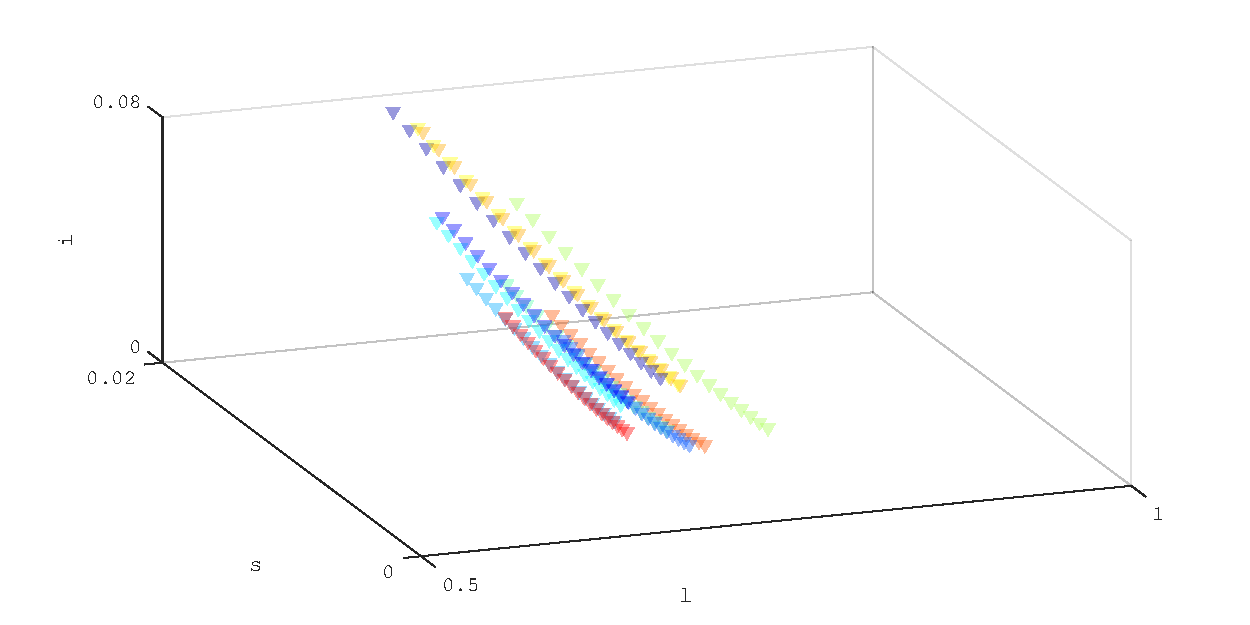
\includegraphics[max width=\textwidth]{figs/comp/melcomp_2/ZL.pdf}
 \caption{\hl{caption}}
 \label{fig:ZL}
\end{figure} 

The script started with the same process as melcomp\_1, loading data and computing \gls{MB} chromaticities, along with hypothetical $i_{\text{MB}}$ values. $r_{\text{MB}}$ values, the rod based analogue, were also calculated, although this was done for completeness (again, following the influence of \cite{barrionuevo_contributions_2014}) rather than following a genuine belief that they could be involved.

In addition to the data considered in melcomp\_1, support was added to consider a range of CIE D series illuminants, the Foster et al. hyperspectral images of natural scenes and the Smith-Pokorny fundamentals.

The CIE D-series illuminants allowed for a smaller and more controlled dataset, the Foster et al. data allowed for a more realistic distribution of reflectances and the Smith-Pokorny fundamentals allowed for a technically `correct' \gls{MB} diagram (before I knew about CIE 170-2:2015 \cite{cie_cie_2015}).

The key finding at this stage was that there is a perspective upon a three-dimensional point cloud ($[l_{\text{MB}},s_{\text{MB}},i_{\text{MB}}]$) from which points from like objects clustered well, such as in figure \ref{fig:viewpoint}. This property shows that there is at least one transformation such that the points could be projected upon a two-dimensional plane where the illuminant dependence was greatly reduced whilst the inter-object chromatic relationships were retained. 

\begin{figure}[htbp]
 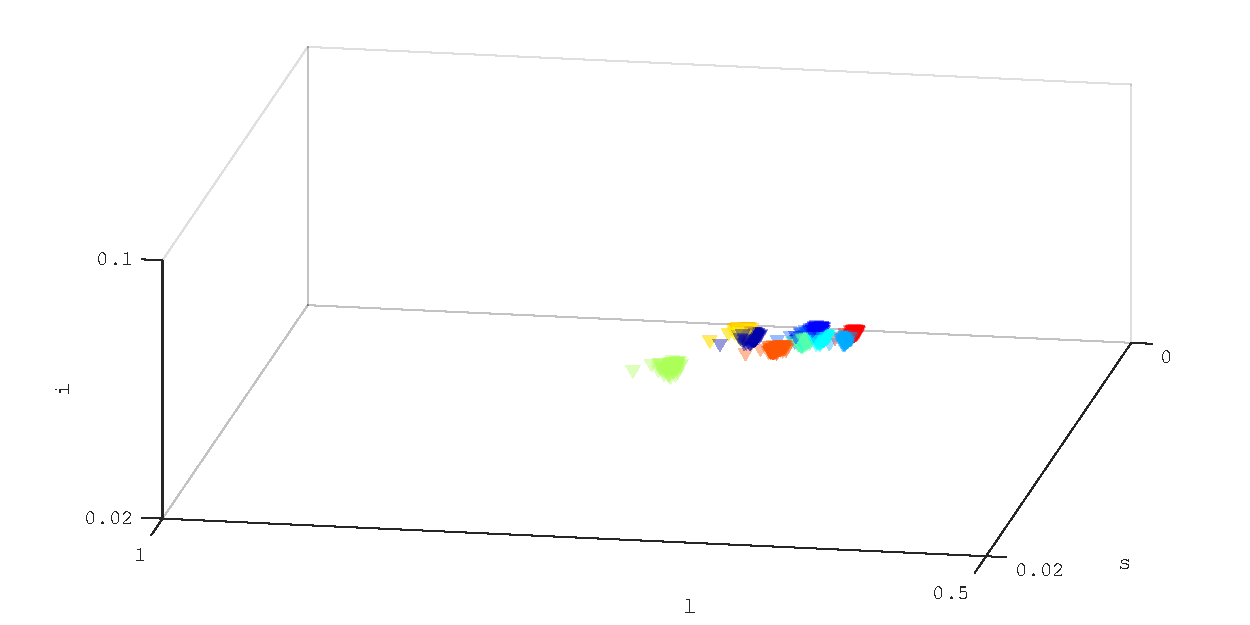
\includegraphics[max width=\textwidth]{figs/comp/melcomp_2_caller/viewpoint.pdf}
 \caption{Figure \ref{fig:ZL} rotated to a perspective where it can be seen that the points project upon a two-dimensional plane in a clustered fashion whilst not degrading to a line within that space.}
 \label{fig:viewpoint}
\end{figure} 

Note that such a perspective would not be possible for a space where the third dimension were a duplicate of the first or second, since in this case all points would lie upon a plane. This would be the case in circumstances where a corrective signal too closely resembled the visual signals.

Following this, a range of speculative transformations were performed, to demonstrate the types of transformation that could be used to transform colour signals to illuminant-independent colour signals. A rotational transformation was successful (analogous to changing the perspective as in figure \ref{fig:viewpoint}) and additionally a weighted additive model was found to be more-or-less successful. No satisfactory model was found where a purely multiplicative transformation was applied.

Thinking about a corrective signal as an additional dimension upon a \gls{MB} chromaticity space allows for consideration of requisite or desirable properties that this third signal should imbue upon the three-dimensional cloud of points. I have identified one requisite property, and one desirable property. 

The requisite property for such a signal, as already suggested, is that it should differ from other chromatic signals enough to allow for the point cloud of chromatic points to be significantly \emph{non-planar}. This in turn allows for a projection upon two-dimensional space which has the potential to be illuminant-invariant.

The desirable property is that it should be \emph{roughly monotonic} with respect to other chromatic signals. This allows a one-to-one mapping of colour signals to illuminant-independent colour signals, where a non-monotonic relationship does not necessarily do so. This is not a strict requirement, since the corrective function only needs to be one directional, but non-monotonicity would exclude simple transforms (such as linear additive or rotational).

The next stage was to search for the underlying reason for the relative success of these transforms. One potential lead is a curious regularity at the lower wavelengths of the reflectance spectrum of many natural objects. In figure \ref{fig:plateau} it can be seen that there is a plateau in the relative spectral reflectances of some natural objects (a subset of the Vrhel reflectances) between roughly 430nm and 480nm, with relatively small deviations within 400nm to 500nm. Another way to visualise this is to calculate the correlation between points on the reflectance function. Such a calculation was performed initially on the Foster data, and then on three other datasets. See figure \ref{fig:foster} and \ref{fig:others} respectively.

\begin{figure}[htbp]
 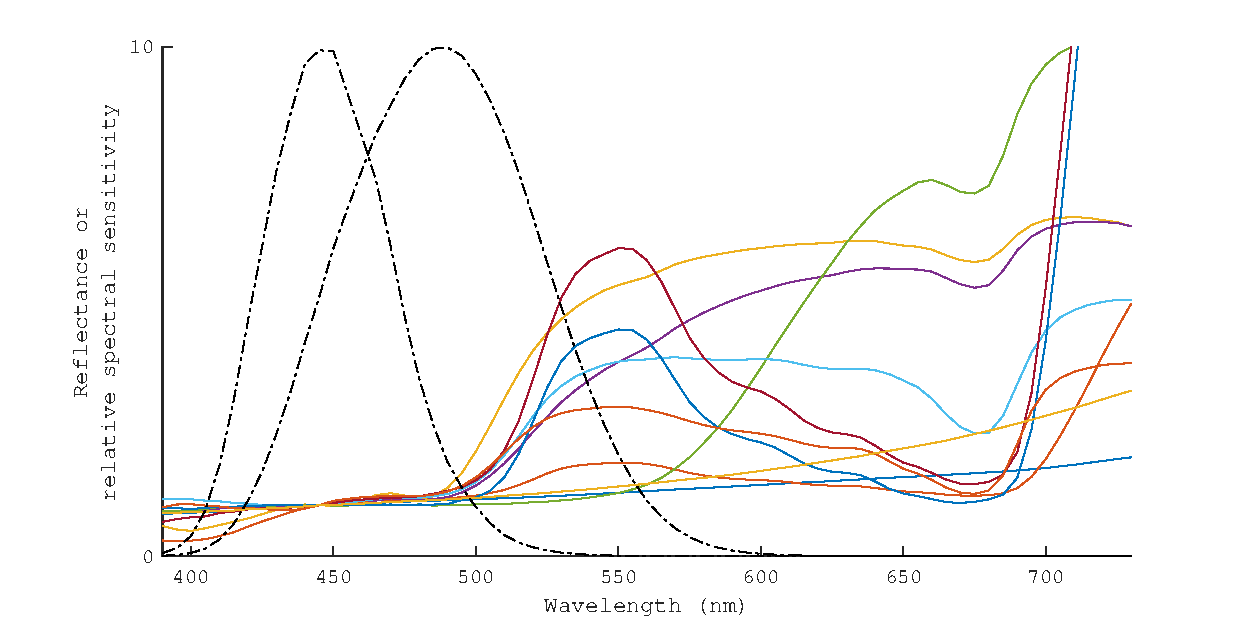
\includegraphics[max width=\textwidth]{figs/comp/melcomp_2_caller/plateau.pdf}
 \caption{The spectral reflectance functions of a subset of the Vrhel reflectances (solid lines), normalised at the peak of s-cone sensitivity, with the spectral sensitivity of s-cones and melanopsin overlaid (dot-dashed lines).}
 \label{fig:plateau}
\end{figure} 

\begin{figure}[htbp]
 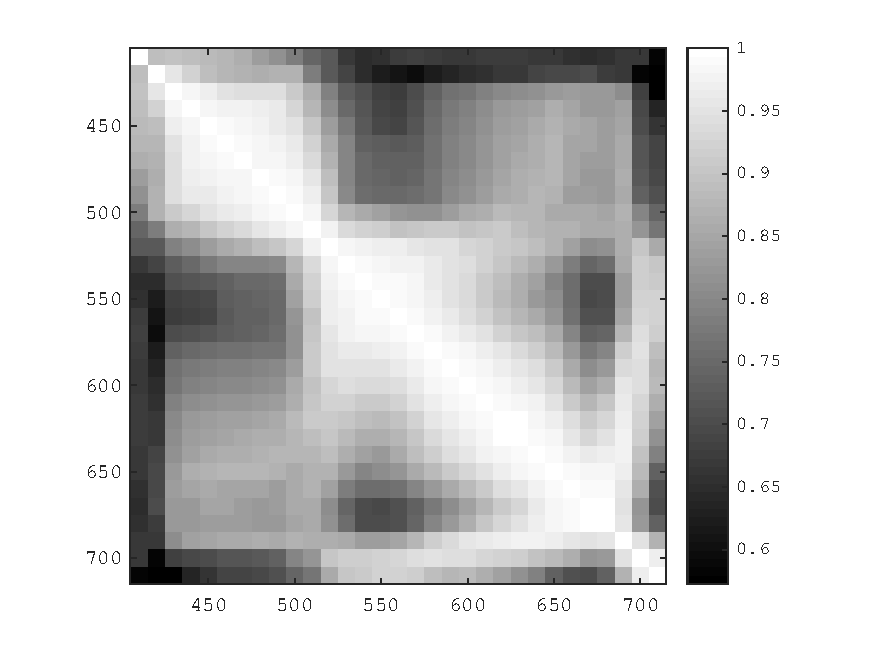
\includegraphics[max width=\textwidth]{figs/comp/nat_cor/foster.pdf}
 \caption{\hl{caption}}
 \label{fig:foster}
\end{figure} 

\begin{figure}[htbp]
 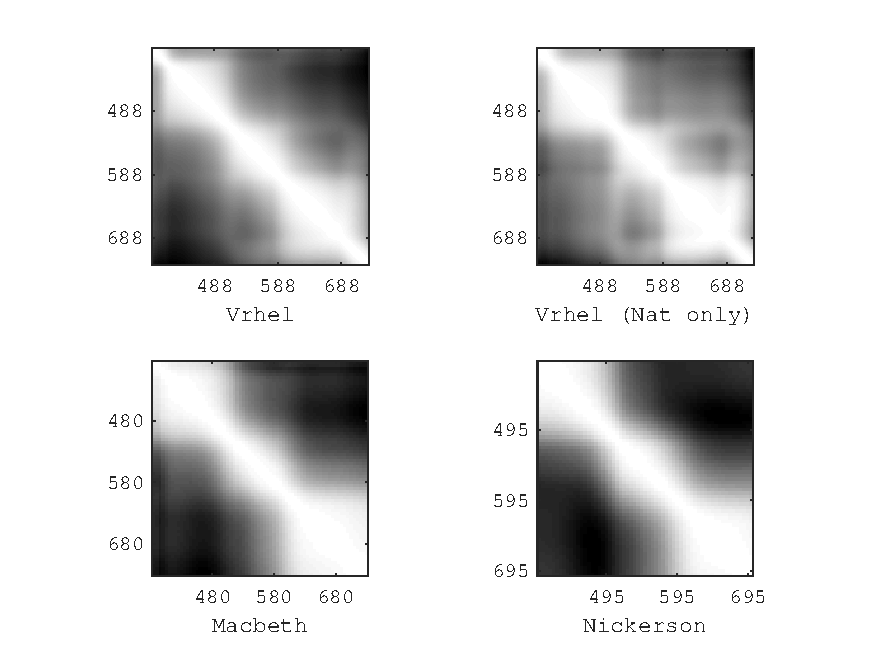
\includegraphics[max width=\textwidth]{figs/comp/nat_cor/others.pdf}
 \caption{\hl{caption}}
 \label{fig:others}
\end{figure} 

An interesting advantage could be made of this regularity. Assume a simpler situation where there were two points on the spectrum of the reflectance functions of a set of natural objects which were always the same as eachother (perfect correlation). Sensors of appropriately narrow spectral sensitivity, placed at these two points on the spectrum would always register corresponding signals. Considering that the second principal component of daylight variability is a broad skew, any difference in the signals from two such receptors could be used fairly reliably to sense the contribution of this second component in any single condition. This explains the relative effectiveness of an $i_{MB}$ in correcting an $s_{MB}$ signal, but the logic for how it corrects an $l_{MB}$ signal is slightly trickier.

This work was presented as a poster at the \emph{Visual Neuroscience Summer School} in 2018 as a poster, which has not been made publicly available.